% Source of the figure diameter-two-structure.pdf (structure of the cut C in the proof of the theorem on graphs of
% diameter two: the sets I, J, K with u in K and v in J; the edges counted in the estimate of |C| are red).
% Compile with pdfLaTeX; the PDF is included in the manuscript at its natural size.
\documentclass[tikz,border=1pt]{standalone}
\usepackage[T1]{fontenc}
\usepackage{stix}
\pdfinfoomitdate=1 \pdftrailerid{} \pdfsuppressptexinfo=-1
\usetikzlibrary{calc}
\definecolor{threadred}{RGB}{200,40,40}
\begin{document}
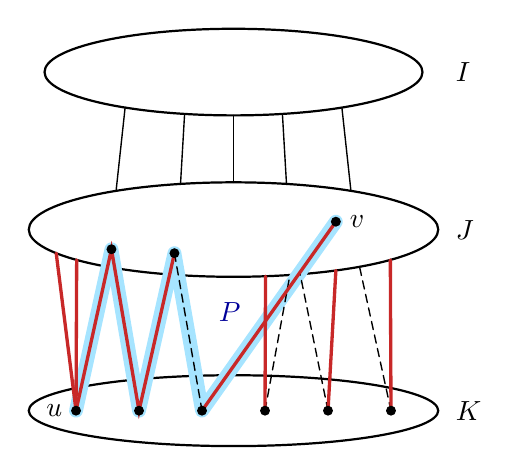
\begin{tikzpicture}[x=1cm, y=1cm,
    set/.style={line width=0.8pt},
    edge/.style={line width=0.5pt, line cap=round},
    other/.style={edge, densely dashed},
    counted/.style={line width=1.2pt, line cap=round, threadred},
    path/.style={line width=5pt, line cap=round, line join=round, blue!30!cyan!35!white}]
  \coordinate (I) at (2.6,4.6);
  \coordinate (J) at (2.6,2.6);
  \coordinate (K) at (2.6,0.3);
  % the three sets; L is empty
  \draw[set] (I) ellipse[x radius=2.4, y radius=0.55];
  \draw[set] (J) ellipse[x radius=2.6, y radius=0.6];
  \draw[set] (K) ellipse[x radius=2.6, y radius=0.45];
  \node[anchor=west] at (5.3,4.6) {$I$};
  \node[anchor=west] at (5.3,2.6) {$J$};
  \node[anchor=west] at (5.3,0.3) {$K$};
  % edges between I and J (not in the cut)
  \foreach \a/\b in {235/125, 255/105, 270/90, 285/75, 305/55}
    \draw[edge] ($(I)+(\a:2.4 and 0.55)$) -- ($(J)+(\b:2.6 and 0.6)$);
  % vertices of K: u, the third vertex x of P, and four further vertices
  \coordinate (u)  at (0.6,0.3);
  \coordinate (x)  at (1.4,0.3);
  \coordinate (k3) at (2.2,0.3);
  \coordinate (k4) at (3.0,0.3);
  \coordinate (k5) at (3.8,0.3);
  \coordinate (k6) at (4.6,0.3);
  % the second and the fourth vertex of P, and v, in J
  \coordinate (y1) at (1.05,2.35);
  \coordinate (y2) at (1.85,2.3);
  \coordinate (v)  at (3.9,2.7);
  % the u-v path P, which lies in the cut C, shaded under the edges
  \draw[path] (u) -- (y1) -- (x) -- (y2) -- (k3) -- (v);
  \node[blue!60!black] at (2.55,1.55) {$P$};
  % cut edges that are not counted
  \draw[other] (y2) -- (k3);
  \draw[other] (k4) -- ($(J)+(-74:2.6 and 0.6)$);
  \draw[other] (k5) -- ($(J)+(-71:2.6 and 0.6)$);
  \draw[other] (k6) -- ($(J)+(-52:2.6 and 0.6)$);
  % counted edges: all edges from u to J, two edges of P at x, one edge at each further vertex of K
  \draw[counted] (u) -- ($(J)+(210:2.6 and 0.6)$);
  \draw[counted] (u) -- ($(J)+(220:2.6 and 0.6)$);
  \draw[counted] (u) -- (y1) -- (x) -- (y2);
  \draw[counted] (k3) -- (v);
  \draw[counted] (k4) -- ($(J)+(-81:2.6 and 0.6)$);
  \draw[counted] (k5) -- ($(J)+(-60:2.6 and 0.6)$);
  \draw[counted] (k6) -- ($(J)+(-40:2.6 and 0.6)$);
  \foreach \p in {u, x, k3, k4, k5, k6, y1, y2, v}
    \fill (\p) circle[radius=1.8pt];
  \node[left=1.5pt] at (u) {$u$};
  \node[right=1.5pt] at (v) {$v$};
\end{tikzpicture}
\end{document}
